%!TEX TS-program = xelatex
\documentclass[notes,12pt, aspectratio=169]{beamer}

\usepackage{amsmath,amsfonts,amssymb,amsthm,mathtools}  % пакеты для математики

\usepackage[english, russian]{babel} % выбор языка для документа
\usepackage[utf8]{inputenc} % задание utf8 кодировки исходного tex файла
\usepackage[X2,T2A]{fontenc}        % кодировка

\usepackage{fontspec}         % пакет для подгрузки шрифтов
\setmainfont{Helvetica}  % задаёт основной шрифт документа

% why do we need \newfontfamily:
% http://tex.stackexchange.com/questions/91507/
\newfontfamily{\cyrillicfonttt}{Helvetica}
\newfontfamily{\cyrillicfont}{Helvetica}
\newfontfamily{\cyrillicfontsf}{Helvetica}

\usepackage{unicode-math}     % пакет для установки математического шрифта
% \setmathfont{Neo Euler} % шрифт для математики

\usepackage{polyglossia}      % Пакет, который позволяет подгружать русские буквы
\setdefaultlanguage{russian}  % Основной язык документа
\setotherlanguage{english}    % Второстепенный язык документа

% Шрифт для кода
\setmonofont[Scale=0.85]{Monaco}
\usepackage{verbments}

\usepackage{pgfpages}
% These slides also contain speaker notes. You can print just the slides,
% just the notes, or both, depending on the setting below. Comment out the want
% you want.
%\setbeameroption{hide notes} % Only slide
%\setbeameroption{show only notes} % Only notes
%\setbeameroption{show notes on second screen=right} % Both

\usepackage{array}

\usepackage{tikz}
\usepackage{verbatim}
\setbeamertemplate{note page}{\pagecolor{yellow!5}\insertnote}
\usetikzlibrary{positioning}
\usetikzlibrary{snakes}
\usetikzlibrary{calc}
\usetikzlibrary{arrows}
\usetikzlibrary{decorations.markings}
\usetikzlibrary{shapes.misc}
\usetikzlibrary{matrix,shapes,arrows,fit,tikzmark}

\usepackage{hyperref}
\usepackage{lipsum}
\usepackage{multimedia}
\usepackage{multirow}
\usepackage{dcolumn}
\usepackage{bbm}
\newcolumntype{d}[0]{D{.}{.}{5}}

\usepackage{changepage}
\usepackage{appendixnumberbeamer}
\newcommand{\beginbackup}{
   \newcounter{framenumbervorappendix}
   \setcounter{framenumbervorappendix}{\value{framenumber}}
   \setbeamertemplate{footline}
   {
     \leavevmode%
     \hline
     box{%
       \begin{beamercolorbox}[wd=\paperwidth,ht=2.25ex,dp=1ex,right]{footlinecolor}%
%         \insertframenumber  \hspace*{2ex} 
       \end{beamercolorbox}}%
     \vskip0pt%
   }
 }
\newcommand{\backupend}{
   \addtocounter{framenumbervorappendix}{-\value{framenumber}}
   \addtocounter{framenumber}{\value{framenumbervorappendix}} 
}

% для имитации питоновского синтаксиса 
\newcommand{\pgr}[1]{{\color{green} \textbf{#1}}}


%%%%%%%%%% Работа с картинками %%%%%%%%%
\usepackage{graphicx}                  % Для вставки рисунков
\usepackage{graphics}
\graphicspath{{../images/}}    % можно указать папки с картинками
\usepackage{wrapfig}                   % Обтекание рисунков и таблиц текстом

\usepackage[space]{grffile}
\usepackage{booktabs}

\usepackage{fontawesome5}
\usepackage{bbding}

% These are my colors -- there are many like them, but these ones are mine.
\definecolor{blue}{RGB}{0,114,178}
\definecolor{red}{RGB}{213,94,0}
\definecolor{yellow}{RGB}{240,228,66}
\definecolor{green}{RGB}{0,128, 0}

\hypersetup{
  colorlinks=true,
  linkbordercolor = {white},
  linkcolor = {blue},
  urlcolor= {blue}
}


%% I use a beige off white for my background
\definecolor{MyBackground}{RGB}{255,253,218}

%% Uncomment this if you want to change the background color to something else
%\setbeamercolor{background canvas}{bg=MyBackground}

%% Change the bg color to adjust your transition slide background color!
\newenvironment{transitionframe}{
  \setbeamercolor{background canvas}{bg=yellow}
  \begin{frame}}{
    \end{frame}
}

\setbeamercolor{frametitle}{fg=blue}
\setbeamercolor{title}{fg=black}
\setbeamertemplate{footline}[frame number]
\setbeamertemplate{navigation symbols}{} 
\setbeamertemplate{itemize items}{-}
\setbeamercolor{itemize item}{fg=blue}
\setbeamercolor{itemize subitem}{fg=blue}
\setbeamercolor{enumerate item}{fg=blue}
\setbeamercolor{enumerate subitem}{fg=blue}
\setbeamercolor{button}{bg=MyBackground,fg=blue,}


% If you like road maps, rather than having clutter at the top, have a roadmap show up at the end of each section 
% (and after your introduction)
% Uncomment this is if you want the roadmap!
% \AtBeginSection[]
% {
%    \begin{frame}
%        \frametitle{Roadmap of Talk}
%        \tableofcontents[currentsection]
%    \end{frame}
% }
\setbeamercolor{section in toc}{fg=blue}
\setbeamercolor{subsection in toc}{fg=red}
\setbeamersize{text margin left=1em,text margin right=1em} 

% списки, которые растягиваются на всю величину слайда 
\newenvironment{wideitemize}{\itemize\addtolength{\itemsep}{10pt}}{\enditemize}


\usepackage{xcolor}

% Syntax: \colorboxed[<color model>]{<color specification>}{<math formula>}
\newcommand*{\colorboxed}{}
\def\colorboxed#1#{%
	\colorboxedAux{#1}%
}

\newcommand*{\colorboxedAux}[3]{%
	% #1: optional argument for color model
	% #2: color specification
	% #3: formula
	\begingroup
	\colorlet{cb@saved}{.}%
	\color#1{#2}%
	\boxed{%
		\color{cb@saved}%
		#3%
	}%
	\endgroup
}

\usepackage{pgfplots}
\usepackage{tikz}

\DeclareMathOperator{\logloss}{logloss}

\title[]{\textcolor{blue}{Анализ данных в R}}
\author{Зарманбетов Ахмед и Мидюкин Максим}
\date{\today}

\usepackage{ulem}

\begin{document}

%%% TIKZ STUFF
\tikzset{   
        every picture/.style={remember picture,baseline},
        every node/.style={anchor=base,align=center,outer sep=1.5pt},
        every path/.style={thick},
        }
\newcommand\marktopleft[1]{%
    \tikz[overlay,remember picture] 
        \node (marker-#1-a) at (-.3em,.3em) {};%
}
\newcommand\markbottomright[2]{%
    \tikz[overlay,remember picture] 
        \node (marker-#1-b) at (0em,0em) {};%
}
\tikzstyle{every picture}+=[remember picture] 
\tikzstyle{mybox} =[draw=black, very thick, rectangle, inner sep=10pt, inner ysep=20pt]
\tikzstyle{fancytitle} =[draw=black,fill=red, text=white]
%%%% END TIKZ STUFF

% Title Slide

\begin{frame}
\maketitle
\centering \textbf{\color{blue} Лекция №1:}  Введение в R, обзор курса
\end{frame}

\begin{frame}{План лекции}
\begin{wideitemize}
	
	\item Знакомство

	\item Правила игры
	
	\item Что будем делать
	
	\item R
	
	\item IDE, RStudio
	
	\item Установка нужного софта
	
	\item Интерфейс RStudio
	
	\item Пишем свой первый код :3
		
\end{wideitemize} 
\end{frame}

\begin{transitionframe}
	\begin{center}
		\Huge Знакомство
	\end{center}
\centering 
\includegraphics[scale = 2]{meet.png}
\end{transitionframe}

\begin{frame}{Кто будет вести курс?}
	\begin{minipage}{0.45\textwidth}
		\centering Зарманбетов Ахмед (Ахмедушка)
		
		\centering 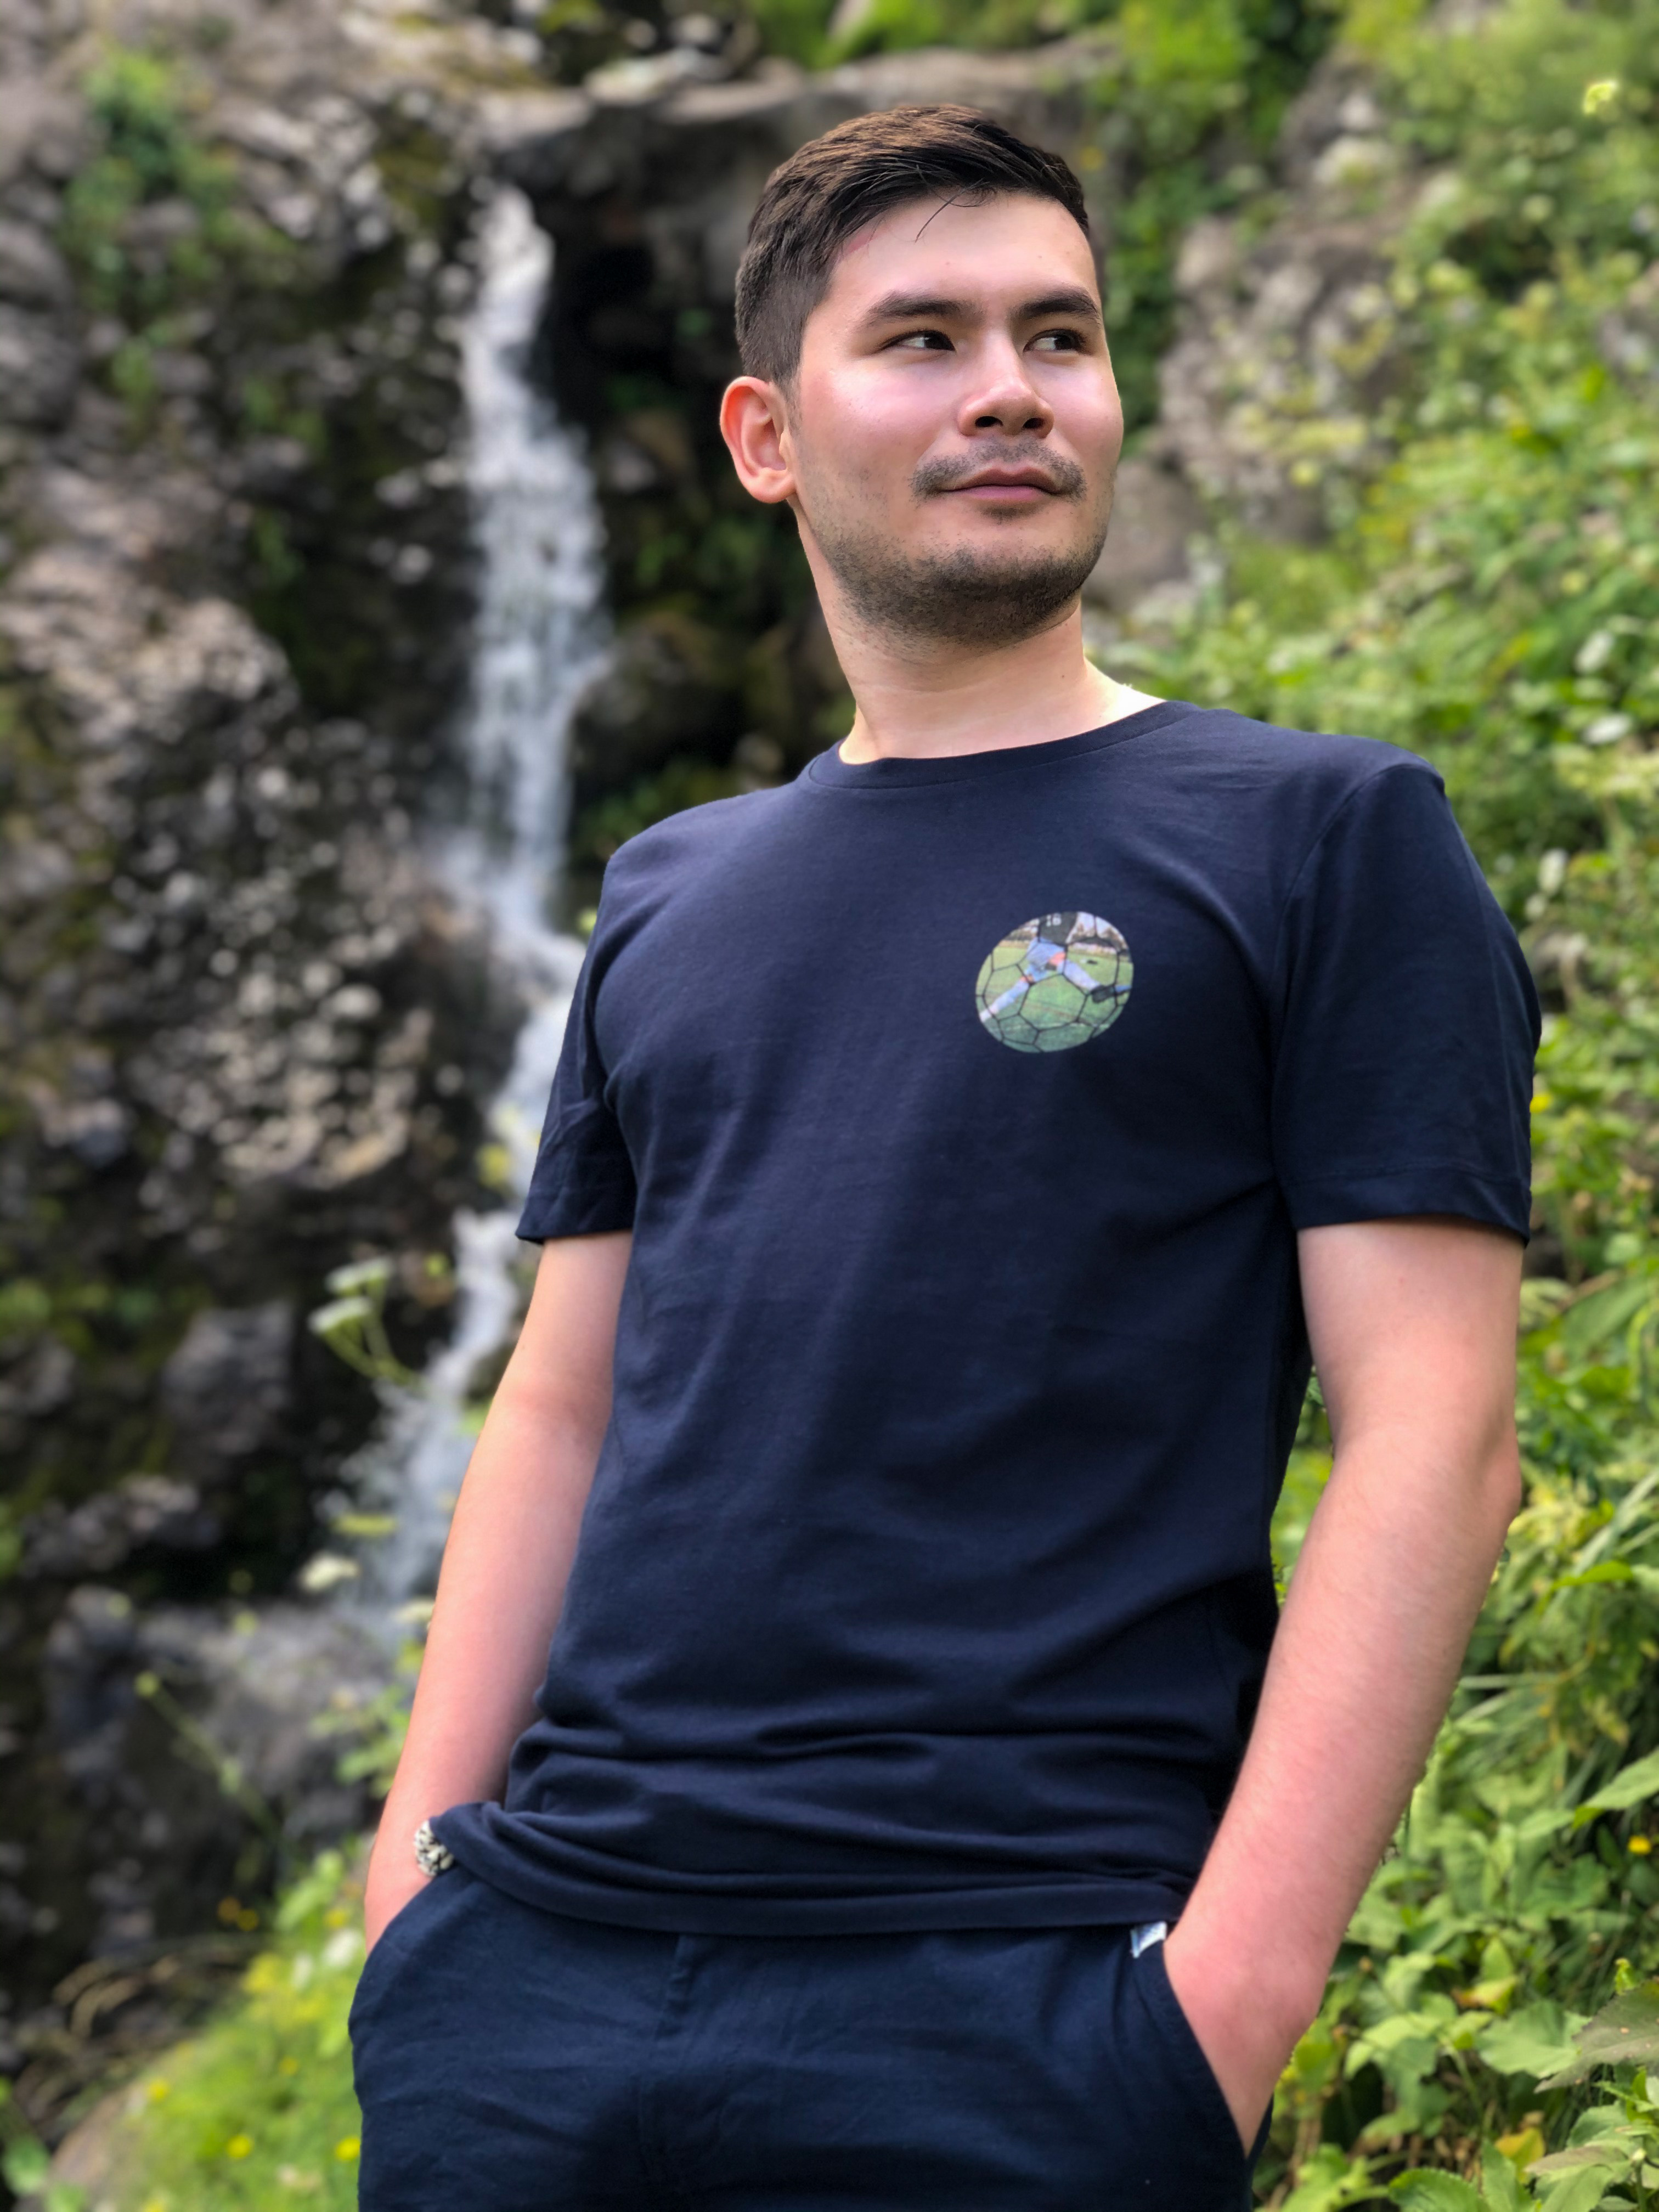
\includegraphics[scale = 0.2]{ahmed.jpg}
	\end{minipage}
	\hfill
	\begin{minipage}{0.45\textwidth}
		\begin{wideitemize}
			
			\item лектор 
			
			\item семинарист группы БСЦ171
			
			\item \faTelegram \: @ahmedushka7
			
			\item \PhoneHandset \: +7(961)-146-70-23
			
		\end{wideitemize} 
	\end{minipage}
\end{frame}

\begin{frame}{Кто будет вести курс?}
	\begin{minipage}{0.45\textwidth}
		\centering Мидюкин Максим
		
		\centering 
\includegraphics[scale = 0.13]{max.jpg}
	\end{minipage}
	\hfill
	\begin{minipage}{0.45\textwidth}
		\begin{wideitemize}
			
			\item семинарист группы БСЦ172
			
			\item \faTelegram \: @midiukin
			
			\item \PhoneHandset  \: +7(926)-932-58-23
			
		\end{wideitemize} 
	\end{minipage}
\end{frame}

\begin{frame}{Контакты}
	\begin{wideitemize}
		
		\item общий канал \hyperref{https://t.me/joinchat/AAAAAEnPA-UXj5C99NFdbA}{}{}{[ссылка]}
		
		\item чат группы  БСЦ171 \hyperref{}{}{}{[ссылка]}
		
		\item чат группы БСЦ172 \hyperref{}{}{}{[ссылка]}
		
	\end{wideitemize} 
\end{frame}

\begin{transitionframe}
	\begin{center}
		\Huge Правила игры
	\end{center}
	\centering 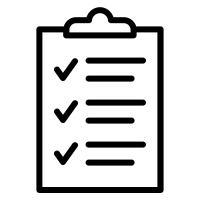
\includegraphics[scale = 0.23]{rules}
\end{transitionframe}

\begin{frame}{Правила игры}
	\begin{wideitemize}
		
		\item что-то непонятно на паре $\Rightarrow$ \alert{ ПЕРЕБЕЙ И СПРОСИ}
		
		\item что-то непонятно дома $\Rightarrow$ \alert{НАПИШИ В ТЕЛЕГРАММ}	
		
		\item обращаться лучше на "ты"	
		
		\item все материалы курса лежат \hyperref{https://ahmedushka7.github.io/R/}{}{}{тут}
	\end{wideitemize} 


\end{frame}

\begin{frame}{Формула оценки}
	\begin{wideitemize}
		
		\item Домашняя работа x3
		
		\item Контрольная работа
		
		\item Письменный экзамен
		
	\end{wideitemize} 

\hfill

\pause 

\[
\text{Оценка} = 0.15 \cdot  \text{ДЗ}_1 + 0.15 \cdot  \text{ДЗ}_2 + 0.15 \cdot  \text{ДЗ}_3 + 0.25 \cdot  \text{КР}  + 0.3 \cdot  \text{ЭКЗ}
\]
\end{frame}


\begin{transitionframe}
	\begin{center}
		\Huge Что будем изучать
	\end{center}
	\centering 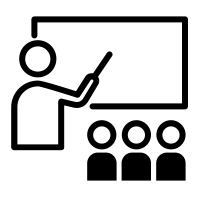
\includegraphics[scale = 0.33]{study.png}
\end{transitionframe}

\begin{frame}{План первой части курса}
	\begin{wideitemize}
		
		\item Основы программирования:
		\begin{itemize}
			\item структуры данных
			\item условные конструкции и циклы
			\item функции 
			\item RMarkdown $-$ правильное оформление документов
		\end{itemize}
		\alert{домашка №1}
		
		\item Работа с данными:
		\begin{itemize}
			\item импорт данных
			\item очистка и преобразование данных
		\end{itemize}		
		\alert{контрольная}
	
	\end{wideitemize} 
	
\end{frame}

\begin{frame}{План второй части курса}
	\begin{wideitemize}
				
		\item Углубленная работа с данными:
		\begin{itemize}
			\item визуализация данных
			\item работа со специальными типами переменных \\
			\alert{домашка №2}
			\item импорт данных из интернета \\
			\alert{домашка №3}
		\end{itemize}	
	
		\item Построение моделей:
		\begin{itemize}
			\item вспоминаем мат. статистику
			\item линейная регрессия
			\item задача кластеризации
		\end{itemize}

		\alert{экзамен}	
		
	\end{wideitemize} 
	
\end{frame}

\begin{transitionframe}
	\centering 
\includegraphics[scale = 0.25]{R.png}
\end{transitionframe}

\begin{frame}{Почему нужен R?}
	\begin{wideitemize}
		
		\item он удобен! 
		
		\item совмещает в себе статистику, первичный анализ и математическое моделирование
		
		\item с ним работают в крупных компаниях

	\end{wideitemize} 
	
\end{frame}

\begin{frame}{Почему нужен R?}
	
	\centering 	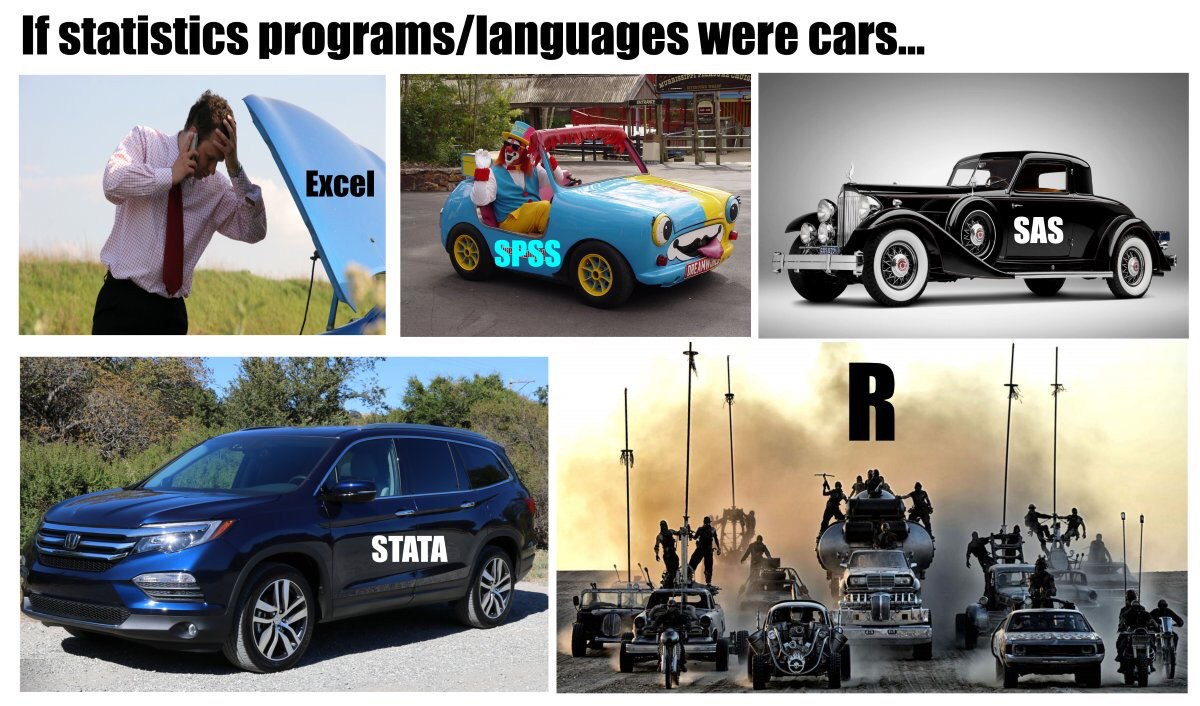
\includegraphics[width=.7\linewidth]{mem.jpeg} 
	
\end{frame}

\begin{transitionframe}
	\begin{center}
		\Huge IDE
	\end{center}
\end{transitionframe}

\begin{frame}{IDE}
	IDE $-$ это интегрированная среда разработки. Говоря простым языком, это удобная программа, которая позволяет вам работать с языком и получать наглядные результаты. Мы будем использовать RStudio 
	
\begin{columns}[T] % align columns
	\begin{column}{.33\textwidth}
		\mbox{ } \\
		\mbox{ } \\
		\mbox{ } \\
		\mbox{ } \\
		\centering 	
\includegraphics[width=.6\linewidth]{jupyter.png} 
	\end{column}%
	\hfill%
	\begin{column}{.33\textwidth}
		\mbox{ } \\
		\mbox{ } \\
		\mbox{ } \\
		\centering 	
\includegraphics[width=.7\linewidth]{rstudio1.png} 		
	\end{column}%
	\hfill%
	\begin{column}{.33\textwidth}
		\centering 	
\includegraphics[width=.6\linewidth]{rkward.png} \\
	\end{column}%
\end{columns}
\end{frame}

\begin{transitionframe}
	\begin{center}
		\Huge Установка нужного софта
	\end{center}
	\centering 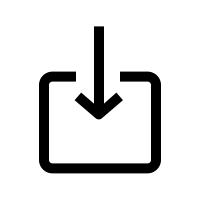
\includegraphics[scale = 0.25]{install.png}
\end{transitionframe}

\begin{frame}{Установка}
	Очень подробное описание установки R и RStudio на любую ОС можно найти \hyperref{https://ahmedushka7.github.io/R/}{}{}{на странице курса.}
\end{frame}

\begin{transitionframe}
	\centering 
\includegraphics[scale = 0.1]{rstudio.png}
\end{transitionframe}

\begin{frame}{Интерфейс RStudio}
	\centering 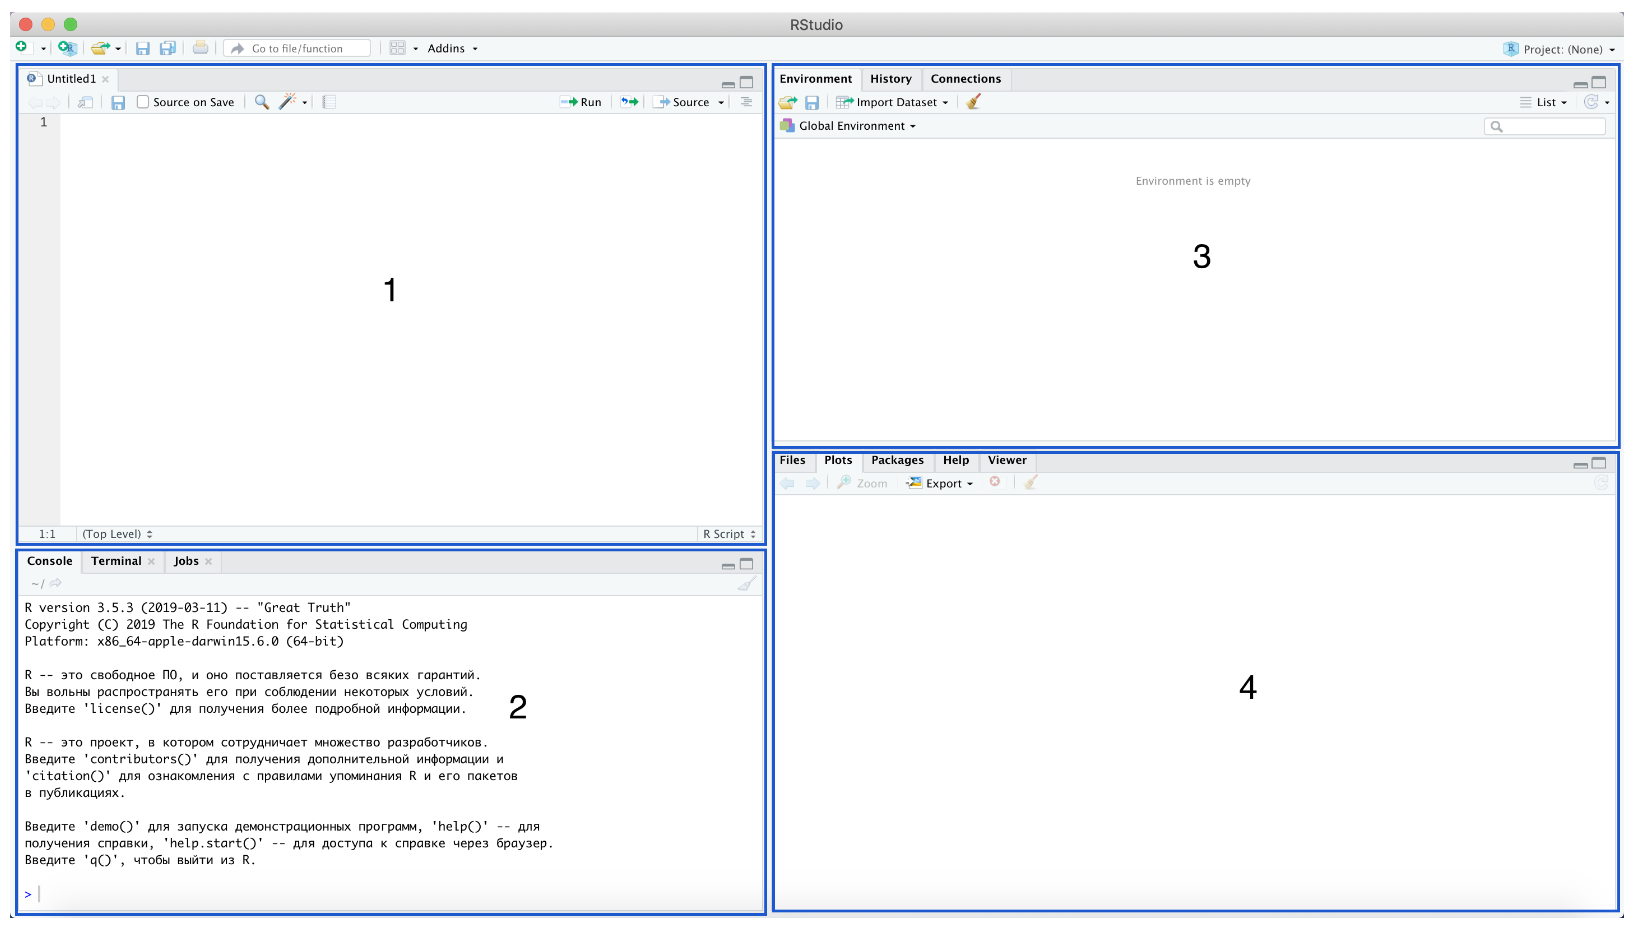
\includegraphics[scale = 0.45]{face.png}
\end{frame}


\begin{transitionframe}
	\begin{center}
		\Huge Пишем свой первый код :3
	\end{center}
\end{transitionframe}

\end{document}

